\documentclass[1p]{elsarticle_modified}
%\bibliographystyle{elsarticle-num}

%\usepackage[colorlinks]{hyperref}
%\usepackage{abbrmath_seonhwa} %\Abb, \Ascr, \Acal ,\Abf, \Afrak
\usepackage{amsfonts}
\usepackage{amssymb}
\usepackage{amsmath}
\usepackage{amsthm}
\usepackage{scalefnt}
\usepackage{amsbsy}
\usepackage{kotex}
\usepackage{caption}
\usepackage{subfig}
\usepackage{color}
\usepackage{graphicx}
\usepackage{xcolor} %% white, black, red, green, blue, cyan, magenta, yellow
\usepackage{float}
\usepackage{setspace}
\usepackage{hyperref}

\usepackage{tikz}
\usetikzlibrary{arrows}

\usepackage{multirow}
\usepackage{array} % fixed length table
\usepackage{hhline}

%%%%%%%%%%%%%%%%%%%%%
\makeatletter
\renewcommand*\env@matrix[1][\arraystretch]{%
	\edef\arraystretch{#1}%
	\hskip -\arraycolsep
	\let\@ifnextchar\new@ifnextchar
	\array{*\c@MaxMatrixCols c}}
\makeatother %https://tex.stackexchange.com/questions/14071/how-can-i-increase-the-line-spacing-in-a-matrix
%%%%%%%%%%%%%%%

\usepackage[normalem]{ulem}

\newcommand{\msout}[1]{\ifmmode\text{\sout{\ensuremath{#1}}}\else\sout{#1}\fi}
%SOURCE: \msout is \stkout macro in https://tex.stackexchange.com/questions/20609/strikeout-in-math-mode

\newcommand{\cancel}[1]{
	\ifmmode
	{\color{red}\msout{#1}}
	\else
	{\color{red}\sout{#1}}
	\fi
}

\newcommand{\add}[1]{
	{\color{blue}\uwave{#1}}
}

\newcommand{\replace}[2]{
	\ifmmode
	{\color{red}\msout{#1}}{\color{blue}\uwave{#2}}
	\else
	{\color{red}\sout{#1}}{\color{blue}\uwave{#2}}
	\fi
}

\newcommand{\Sol}{\mathcal{S}} %segment
\newcommand{\D}{D} %diagram
\newcommand{\A}{\mathcal{A}} %arc


%%%%%%%%%%%%%%%%%%%%%%%%%%%%%5 test

\def\sl{\operatorname{\textup{SL}}(2,\Cbb)}
\def\psl{\operatorname{\textup{PSL}}(2,\Cbb)}
\def\quan{\mkern 1mu \triangleright \mkern 1mu}

\theoremstyle{definition}
\newtheorem{thm}{Theorem}[section]
\newtheorem{prop}[thm]{Proposition}
\newtheorem{lem}[thm]{Lemma}
\newtheorem{ques}[thm]{Question}
\newtheorem{cor}[thm]{Corollary}
\newtheorem{defn}[thm]{Definition}
\newtheorem{exam}[thm]{Example}
\newtheorem{rmk}[thm]{Remark}
\newtheorem{alg}[thm]{Algorithm}

\newcommand{\I}{\sqrt{-1}}
\begin{document}

%\begin{frontmatter}
%
%\title{Boundary parabolic representations of knots up to 8 crossings}
%
%%% Group authors per affiliation:
%\author{Yunhi Cho} 
%\address{Department of Mathematics, University of Seoul, Seoul, Korea}
%\ead{yhcho@uos.ac.kr}
%
%
%\author{Seonhwa Kim} %\fnref{s_kim}}
%\address{Center for Geometry and Physics, Institute for Basic Science, Pohang, 37673, Korea}
%\ead{ryeona17@ibs.re.kr}
%
%\author{Hyuk Kim}
%\address{Department of Mathematical Sciences, Seoul National University, Seoul 08826, Korea}
%\ead{hyukkim@snu.ac.kr}
%
%\author{Seokbeom Yoon}
%\address{Department of Mathematical Sciences, Seoul National University, Seoul, 08826,  Korea}
%\ead{sbyoon15@snu.ac.kr}
%
%\begin{abstract}
%We find all boundary parabolic representation of knots up to 8 crossings.
%
%\end{abstract}
%\begin{keyword}
%    \MSC[2010] 57M25 
%\end{keyword}
%
%\end{frontmatter}

%\linenumbers
%\tableofcontents
%
\newcommand\colored[1]{\textcolor{white}{\rule[-0.35ex]{0.8em}{1.4ex}}\kern-0.8em\color{red} #1}%
%\newcommand\colored[1]{\textcolor{white}{ #1}\kern-2.17ex	\textcolor{white}{ #1}\kern-1.81ex	\textcolor{white}{ #1}\kern-2.15ex\color{red}#1	}

{\Large $\underline{11n_{32}~(K11n_{32})}$}

\setlength{\tabcolsep}{10pt}
\renewcommand{\arraystretch}{1.6}
\vspace{1cm}\begin{tabular}{m{100pt}>{\centering\arraybackslash}m{274pt}}
\multirow{5}{120pt}{
	\centering
	\includegraphics[width=112pt]{../../../GIT/diagram.site/Diagrams/png/648_11n_32.png}\\
\ \ \ A knot diagram\footnotemark}&
\allowdisplaybreaks
\textbf{Linearized knot diagam} \\
\cline{2-2}
 &
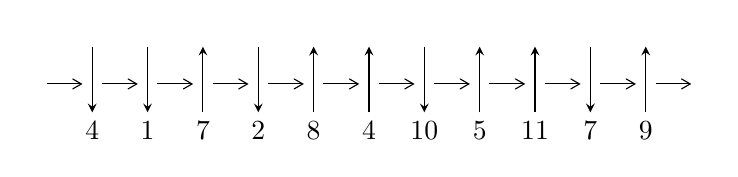
\begin{tikzpicture}[x=20pt, y=17pt]
	% nodes
	\node (C0) at (0, 0) {};
	\node (C1) at (1, 0) {};
	\node (C1U) at (1, +1) {};
	\node (C1D) at (1, -1) {4};

	\node (C2) at (2, 0) {};
	\node (C2U) at (2, +1) {};
	\node (C2D) at (2, -1) {1};

	\node (C3) at (3, 0) {};
	\node (C3U) at (3, +1) {};
	\node (C3D) at (3, -1) {7};

	\node (C4) at (4, 0) {};
	\node (C4U) at (4, +1) {};
	\node (C4D) at (4, -1) {2};

	\node (C5) at (5, 0) {};
	\node (C5U) at (5, +1) {};
	\node (C5D) at (5, -1) {8};

	\node (C6) at (6, 0) {};
	\node (C6U) at (6, +1) {};
	\node (C6D) at (6, -1) {4};

	\node (C7) at (7, 0) {};
	\node (C7U) at (7, +1) {};
	\node (C7D) at (7, -1) {10};

	\node (C8) at (8, 0) {};
	\node (C8U) at (8, +1) {};
	\node (C8D) at (8, -1) {5};

	\node (C9) at (9, 0) {};
	\node (C9U) at (9, +1) {};
	\node (C9D) at (9, -1) {11};

	\node (C10) at (10, 0) {};
	\node (C10U) at (10, +1) {};
	\node (C10D) at (10, -1) {7};

	\node (C11) at (11, 0) {};
	\node (C11U) at (11, +1) {};
	\node (C11D) at (11, -1) {9};
	\node (C12) at (12, 0) {};

	% arrows
	\draw[->,>={angle 60}]
	(C0) edge (C1) (C1) edge (C2) (C2) edge (C3) (C3) edge (C4) (C4) edge (C5) (C5) edge (C6) (C6) edge (C7) (C7) edge (C8) (C8) edge (C9) (C9) edge (C10) (C10) edge (C11) (C11) edge (C12) ;	\draw[->,>=stealth]
	(C1U) edge (C1D) (C2U) edge (C2D) (C3D) edge (C3U) (C4U) edge (C4D) (C5D) edge (C5U) (C6D) edge (C6U) (C7U) edge (C7D) (C8D) edge (C8U) (C9D) edge (C9U) (C10U) edge (C10D) (C11D) edge (C11U) ;
	\end{tikzpicture} \\
\hhline{~~} \\& 
\textbf{Solving Sequence} \\ \cline{2-2} 
 &
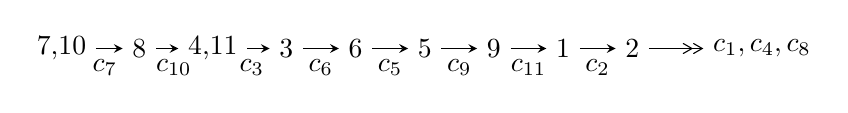
\begin{tikzpicture}[x=25pt, y=7pt]
	% node
	\node (A0) at (-1/8, 0) {7,10};
	\node (A1) at (1, 0) {8};
	\node (A2) at (33/16, 0) {4,11};
	\node (A3) at (25/8, 0) {3};
	\node (A4) at (33/8, 0) {6};
	\node (A5) at (41/8, 0) {5};
	\node (A6) at (49/8, 0) {9};
	\node (A7) at (57/8, 0) {1};
	\node (A8) at (65/8, 0) {2};
	\node (C1) at (1/2, -1) {$c_{7}$};
	\node (C2) at (3/2, -1) {$c_{10}$};
	\node (C3) at (21/8, -1) {$c_{3}$};
	\node (C4) at (29/8, -1) {$c_{6}$};
	\node (C5) at (37/8, -1) {$c_{5}$};
	\node (C6) at (45/8, -1) {$c_{9}$};
	\node (C7) at (53/8, -1) {$c_{11}$};
	\node (C8) at (61/8, -1) {$c_{2}$};
	\node (A9) at (10, 0) {$c_{1},c_{4},c_{8}$};

	% edge
	\draw[->,>=stealth]	
	(A0) edge (A1) (A1) edge (A2) (A2) edge (A3) (A3) edge (A4) (A4) edge (A5) (A5) edge (A6) (A6) edge (A7) (A7) edge (A8) ;
	\draw[->>,>={angle 60}]	
	(A8) edge (A9);
\end{tikzpicture} \\ 

\end{tabular} \\

\footnotetext{
The image of knot diagram is generated by the software ``\textbf{Draw programme}" developed by Andrew Bartholomew(\url{http://www.layer8.co.uk/maths/draw/index.htm\#Running-draw}), where we modified some parts for our purpose(\url{https://github.com/CATsTAILs/LinksPainter}).
}\phantom \\ \newline 
\centering \textbf{Ideals for irreducible components\footnotemark of $X_{\text{par}}$} 
 
\begin{align*}
I^u_{1}&=\langle 
19332758361 u^{37}+38734840795 u^{36}+\cdots+237713005774 b-28141164923,\\
\phantom{I^u_{1}}&\phantom{= \langle  }-1588415703 u^{37}-117670058213 u^{36}+\cdots+237713005774 a+597215892201,\\
\phantom{I^u_{1}}&\phantom{= \langle  }u^{38}+2 u^{37}+\cdots-3 u+1\rangle \\
I^u_{2}&=\langle 
b,\;- u^3-2 u^2+a-2 u,\;u^4+u^3+u^2+1\rangle \\
\\
\end{align*}
\raggedright * 2 irreducible components of $\dim_{\mathbb{C}}=0$, with total 42 representations.\\
\footnotetext{All coefficients of polynomials are rational numbers. But the coefficients are sometimes approximated in decimal forms when there is not enough margin.}
\newpage
\renewcommand{\arraystretch}{1}
\centering \section*{I. $I^u_{1}= \langle 1.93\times10^{10} u^{37}+3.87\times10^{10} u^{36}+\cdots+2.38\times10^{11} b-2.81\times10^{10},\;-1.59\times10^{9} u^{37}-1.18\times10^{11} u^{36}+\cdots+2.38\times10^{11} a+5.97\times10^{11},\;u^{38}+2 u^{37}+\cdots-3 u+1 \rangle$}
\flushleft \textbf{(i) Arc colorings}\\
\begin{tabular}{m{7pt} m{180pt} m{7pt} m{180pt} }
\flushright $a_{7}=$&$\begin{pmatrix}1\\0\end{pmatrix}$ \\
\flushright $a_{10}=$&$\begin{pmatrix}0\\u\end{pmatrix}$ \\
\flushright $a_{8}=$&$\begin{pmatrix}1\\u^2\end{pmatrix}$ \\
\flushright $a_{4}=$&$\begin{pmatrix}0.00668207 u^{37}+0.495009 u^{36}+\cdots+2.86415 u-2.51234\\-0.0813281 u^{37}-0.162948 u^{36}+\cdots+1.48580 u+0.118383\end{pmatrix}$ \\
\flushright $a_{11}=$&$\begin{pmatrix}- u\\u\end{pmatrix}$ \\
\flushright $a_{3}=$&$\begin{pmatrix}0.0880102 u^{37}+0.657957 u^{36}+\cdots+1.37835 u-2.63072\\-0.0813281 u^{37}-0.162948 u^{36}+\cdots+1.48580 u+0.118383\end{pmatrix}$ \\
\flushright $a_{6}=$&$\begin{pmatrix}0.398557 u^{37}+0.370367 u^{36}+\cdots+1.42515 u-1.31533\\0.825719 u^{37}+1.65248 u^{36}+\cdots-2.59421 u+0.826766\end{pmatrix}$ \\
\flushright $a_{5}=$&$\begin{pmatrix}0.397978 u^{37}-0.632706 u^{36}+\cdots+2.34056 u-1.71535\\1.43070 u^{37}+2.85936 u^{36}+\cdots-5.59937 u+1.82868\end{pmatrix}$ \\
\flushright $a_{9}=$&$\begin{pmatrix}- u^3\\u^3+u\end{pmatrix}$ \\
\flushright $a_{1}=$&$\begin{pmatrix}- u^5- u\\u^5+u^3+u\end{pmatrix}$ \\
\flushright $a_{2}=$&$\begin{pmatrix}0.196219 u^{37}+0.547563 u^{36}+\cdots+2.31038 u-3.08666\\0.243984 u^{37}+0.488844 u^{36}+\cdots+0.542588 u+0.644851\end{pmatrix}$\\ \flushright $a_{2}=$&$\begin{pmatrix}0.196219 u^{37}+0.547563 u^{36}+\cdots+2.31038 u-3.08666\\0.243984 u^{37}+0.488844 u^{36}+\cdots+0.542588 u+0.644851\end{pmatrix}$\\&\end{tabular}
\flushleft \textbf{(ii) Obstruction class $= -1$}\\~\\
\flushleft \textbf{(iii) Cusp Shapes $= -\frac{159159118679}{118856502887} u^{37}-\frac{28323238958}{118856502887} u^{36}+\cdots+\frac{412587165626}{118856502887} u-\frac{634600057867}{118856502887}$}\\~\\
\newpage\renewcommand{\arraystretch}{1}
\flushleft \textbf{(iv) u-Polynomials at the component}\newline \\
\begin{tabular}{m{50pt}|m{274pt}}
Crossings & \hspace{64pt}u-Polynomials at each crossing \\
\hline $$\begin{aligned}c_{1},c_{4}\end{aligned}$$&$\begin{aligned}
&u^{38}-5 u^{37}+\cdots+u+1
\end{aligned}$\\
\hline $$\begin{aligned}c_{2}\end{aligned}$$&$\begin{aligned}
&u^{38}+15 u^{37}+\cdots-81 u+1
\end{aligned}$\\
\hline $$\begin{aligned}c_{3},c_{6}\end{aligned}$$&$\begin{aligned}
&u^{38}+5 u^{37}+\cdots+104 u+16
\end{aligned}$\\
\hline $$\begin{aligned}c_{5},c_{8}\end{aligned}$$&$\begin{aligned}
&u^{38}+2 u^{37}+\cdots+u+1
\end{aligned}$\\
\hline $$\begin{aligned}c_{7},c_{10}\end{aligned}$$&$\begin{aligned}
&u^{38}-2 u^{37}+\cdots+3 u+1
\end{aligned}$\\
\hline $$\begin{aligned}c_{9},c_{11}\end{aligned}$$&$\begin{aligned}
&u^{38}-14 u^{37}+\cdots-7 u+1
\end{aligned}$\\
\hline
\end{tabular}\\~\\
\newpage\renewcommand{\arraystretch}{1}
\flushleft \textbf{(v) Riley Polynomials at the component}\newline \\
\begin{tabular}{m{50pt}|m{274pt}}
Crossings & \hspace{64pt}Riley Polynomials at each crossing \\
\hline $$\begin{aligned}c_{1},c_{4}\end{aligned}$$&$\begin{aligned}
&y^{38}-15 y^{37}+\cdots+81 y+1
\end{aligned}$\\
\hline $$\begin{aligned}c_{2}\end{aligned}$$&$\begin{aligned}
&y^{38}+21 y^{37}+\cdots-2859 y+1
\end{aligned}$\\
\hline $$\begin{aligned}c_{3},c_{6}\end{aligned}$$&$\begin{aligned}
&y^{38}-27 y^{37}+\cdots-320 y+256
\end{aligned}$\\
\hline $$\begin{aligned}c_{5},c_{8}\end{aligned}$$&$\begin{aligned}
&y^{38}+10 y^{37}+\cdots+7 y+1
\end{aligned}$\\
\hline $$\begin{aligned}c_{7},c_{10}\end{aligned}$$&$\begin{aligned}
&y^{38}+14 y^{37}+\cdots+7 y+1
\end{aligned}$\\
\hline $$\begin{aligned}c_{9},c_{11}\end{aligned}$$&$\begin{aligned}
&y^{38}+22 y^{37}+\cdots+179 y+1
\end{aligned}$\\
\hline
\end{tabular}\\~\\
\newpage\flushleft \textbf{(vi) Complex Volumes and Cusp Shapes}
$$\begin{array}{c|c|c}  
\text{Solutions to }I^u_{1}& \I (\text{vol} + \sqrt{-1}CS) & \text{Cusp shape}\\
 \hline 
\begin{aligned}
u &= \phantom{-}0.832670 + 0.614929 I \\
a &= -0.103257 - 0.153512 I \\
b &= -1.139290 - 0.198092 I\end{aligned}
 & \phantom{-}0.789901 + 0.872417 I & \phantom{-}0.203682 - 1.029460 I \\ \hline\begin{aligned}
u &= \phantom{-}0.832670 - 0.614929 I \\
a &= -0.103257 + 0.153512 I \\
b &= -1.139290 + 0.198092 I\end{aligned}
 & \phantom{-}0.789901 - 0.872417 I & \phantom{-}0.203682 + 1.029460 I \\ \hline\begin{aligned}
u &= \phantom{-}0.524709 + 0.798298 I \\
a &= \phantom{-}1.72507 + 2.99817 I \\
b &= -0.278602 + 0.363866 I\end{aligned}
 & -1.79987 - 1.63683 I & \phantom{-}0.6342 + 22.3814 I \\ \hline\begin{aligned}
u &= \phantom{-}0.524709 - 0.798298 I \\
a &= \phantom{-}1.72507 - 2.99817 I \\
b &= -0.278602 - 0.363866 I\end{aligned}
 & -1.79987 + 1.63683 I & \phantom{-}0.6342 - 22.3814 I \\ \hline\begin{aligned}
u &= -0.878464 + 0.565928 I \\
a &= -0.118175 - 0.080326 I \\
b &= \phantom{-}1.32611 - 0.72615 I\end{aligned}
 & -0.48850 - 8.10053 I & -2.17285 + 4.60397 I \\ \hline\begin{aligned}
u &= -0.878464 - 0.565928 I \\
a &= -0.118175 + 0.080326 I \\
b &= \phantom{-}1.32611 + 0.72615 I\end{aligned}
 & -0.48850 + 8.10053 I & -2.17285 - 4.60397 I \\ \hline\begin{aligned}
u &= -0.628453 + 0.715455 I \\
a &= -1.32808 + 0.68300 I \\
b &= \phantom{-}0.55366 + 1.35876 I\end{aligned}
 & -3.24288 - 0.91080 I & -5.85440 + 2.87226 I \\ \hline\begin{aligned}
u &= -0.628453 - 0.715455 I \\
a &= -1.32808 - 0.68300 I \\
b &= \phantom{-}0.55366 - 1.35876 I\end{aligned}
 & -3.24288 + 0.91080 I & -5.85440 - 2.87226 I \\ \hline\begin{aligned}
u &= -0.638347 + 0.845542 I \\
a &= -1.27115 + 1.10932 I \\
b &= \phantom{-}1.52004 - 0.19492 I\end{aligned}
 & -4.60338 + 2.49292 I & -7.66096 - 3.58742 I \\ \hline\begin{aligned}
u &= -0.638347 - 0.845542 I \\
a &= -1.27115 - 1.10932 I \\
b &= \phantom{-}1.52004 + 0.19492 I\end{aligned}
 & -4.60338 - 2.49292 I & -7.66096 + 3.58742 I\\
 \hline 
 \end{array}$$\newpage$$\begin{array}{c|c|c}  
\text{Solutions to }I^u_{1}& \I (\text{vol} + \sqrt{-1}CS) & \text{Cusp shape}\\
 \hline 
\begin{aligned}
u &= \phantom{-}0.842903 + 0.381952 I \\
a &= -0.152164 - 0.103068 I \\
b &= \phantom{-}1.156070 - 0.287792 I\end{aligned}
 & \phantom{-}0.57801 - 4.07433 I & -1.00107 + 5.21688 I \\ \hline\begin{aligned}
u &= \phantom{-}0.842903 - 0.381952 I \\
a &= -0.152164 + 0.103068 I \\
b &= \phantom{-}1.156070 + 0.287792 I\end{aligned}
 & \phantom{-}0.57801 + 4.07433 I & -1.00107 - 5.21688 I \\ \hline\begin{aligned}
u &= \phantom{-}0.563322 + 0.919944 I \\
a &= -0.76392 - 1.40999 I \\
b &= -0.162866 - 0.630461 I\end{aligned}
 & -1.35379 - 2.75023 I & -1.67570 - 2.67847 I \\ \hline\begin{aligned}
u &= \phantom{-}0.563322 - 0.919944 I \\
a &= -0.76392 + 1.40999 I \\
b &= -0.162866 + 0.630461 I\end{aligned}
 & -1.35379 + 2.75023 I & -1.67570 + 2.67847 I \\ \hline\begin{aligned}
u &= \phantom{-}0.361485 + 0.817539 I \\
a &= -0.685289 - 0.170023 I \\
b &= \phantom{-}0.230395 + 0.298664 I\end{aligned}
 & \phantom{-}0.31225 - 1.54508 I & \phantom{-}2.23777 + 4.87383 I \\ \hline\begin{aligned}
u &= \phantom{-}0.361485 - 0.817539 I \\
a &= -0.685289 + 0.170023 I \\
b &= \phantom{-}0.230395 - 0.298664 I\end{aligned}
 & \phantom{-}0.31225 + 1.54508 I & \phantom{-}2.23777 - 4.87383 I \\ \hline\begin{aligned}
u &= -0.628379 + 0.944326 I \\
a &= \phantom{-}1.065350 + 0.455542 I \\
b &= \phantom{-}0.26079 - 1.59013 I\end{aligned}
 & -2.54932 + 5.85938 I & -3.38157 - 9.01726 I \\ \hline\begin{aligned}
u &= -0.628379 - 0.944326 I \\
a &= \phantom{-}1.065350 - 0.455542 I \\
b &= \phantom{-}0.26079 + 1.59013 I\end{aligned}
 & -2.54932 - 5.85938 I & -3.38157 + 9.01726 I \\ \hline\begin{aligned}
u &= -0.060400 + 1.136280 I \\
a &= \phantom{-}2.28811 - 0.57277 I \\
b &= -1.53818 + 0.08244 I\end{aligned}
 & \phantom{-}7.11789 - 0.13853 I & \phantom{-}5.96603 - 0.12241 I \\ \hline\begin{aligned}
u &= -0.060400 - 1.136280 I \\
a &= \phantom{-}2.28811 + 0.57277 I \\
b &= -1.53818 - 0.08244 I\end{aligned}
 & \phantom{-}7.11789 + 0.13853 I & \phantom{-}5.96603 + 0.12241 I\\
 \hline 
 \end{array}$$\newpage$$\begin{array}{c|c|c}  
\text{Solutions to }I^u_{1}& \I (\text{vol} + \sqrt{-1}CS) & \text{Cusp shape}\\
 \hline 
\begin{aligned}
u &= -0.724985 + 0.458617 I \\
a &= -0.059958 - 0.272456 I \\
b &= -1.32367 + 0.54173 I\end{aligned}
 & \phantom{-}1.89024 - 2.00477 I & \phantom{-}0.55164 + 1.57531 I \\ \hline\begin{aligned}
u &= -0.724985 - 0.458617 I \\
a &= -0.059958 + 0.272456 I \\
b &= -1.32367 - 0.54173 I\end{aligned}
 & \phantom{-}1.89024 + 2.00477 I & \phantom{-}0.55164 - 1.57531 I \\ \hline\begin{aligned}
u &= \phantom{-}0.068191 + 1.190830 I \\
a &= -2.23931 + 0.30504 I \\
b &= \phantom{-}1.45402 - 0.43836 I\end{aligned}
 & \phantom{-}6.16601 - 6.56194 I & \phantom{-}4.09697 + 5.13849 I \\ \hline\begin{aligned}
u &= \phantom{-}0.068191 - 1.190830 I \\
a &= -2.23931 - 0.30504 I \\
b &= \phantom{-}1.45402 + 0.43836 I\end{aligned}
 & \phantom{-}6.16601 + 6.56194 I & \phantom{-}4.09697 - 5.13849 I \\ \hline\begin{aligned}
u &= \phantom{-}0.019048 + 0.780202 I \\
a &= -0.406821 - 0.905002 I \\
b &= -0.275945 + 0.814062 I\end{aligned}
 & \phantom{-}0.77944 - 1.52604 I & \phantom{-}4.36193 + 4.60900 I \\ \hline\begin{aligned}
u &= \phantom{-}0.019048 - 0.780202 I \\
a &= -0.406821 + 0.905002 I \\
b &= -0.275945 - 0.814062 I\end{aligned}
 & \phantom{-}0.77944 + 1.52604 I & \phantom{-}4.36193 - 4.60900 I \\ \hline\begin{aligned}
u &= -0.619321 + 1.057560 I \\
a &= \phantom{-}1.77643 - 1.22273 I \\
b &= -1.62072 - 0.63223 I\end{aligned}
 & \phantom{-}3.58657 + 7.12992 I & \phantom{-}2.46388 - 6.33493 I \\ \hline\begin{aligned}
u &= -0.619321 - 1.057560 I \\
a &= \phantom{-}1.77643 + 1.22273 I \\
b &= -1.62072 + 0.63223 I\end{aligned}
 & \phantom{-}3.58657 - 7.12992 I & \phantom{-}2.46388 + 6.33493 I \\ \hline\begin{aligned}
u &= \phantom{-}0.593324 + 1.105700 I \\
a &= -0.99629 - 1.25159 I \\
b &= \phantom{-}1.233010 + 0.050062 I\end{aligned}
 & \phantom{-}2.77951 - 1.18659 I & \phantom{-}2.30827 - 0.46017 I \\ \hline\begin{aligned}
u &= \phantom{-}0.593324 - 1.105700 I \\
a &= -0.99629 + 1.25159 I \\
b &= \phantom{-}1.233010 - 0.050062 I\end{aligned}
 & \phantom{-}2.77951 + 1.18659 I & \phantom{-}2.30827 + 0.46017 I\\
 \hline 
 \end{array}$$\newpage$$\begin{array}{c|c|c}  
\text{Solutions to }I^u_{1}& \I (\text{vol} + \sqrt{-1}CS) & \text{Cusp shape}\\
 \hline 
\begin{aligned}
u &= -0.876704 + 0.917775 I \\
a &= \phantom{-}0.013016 + 0.303072 I \\
b &= \phantom{-}0.533786 + 0.030166 I\end{aligned}
 & -8.01967 + 3.23855 I & \phantom{-}7.49106 - 4.17157 I \\ \hline\begin{aligned}
u &= -0.876704 - 0.917775 I \\
a &= \phantom{-}0.013016 - 0.303072 I \\
b &= \phantom{-}0.533786 - 0.030166 I\end{aligned}
 & -8.01967 - 3.23855 I & \phantom{-}7.49106 + 4.17157 I \\ \hline\begin{aligned}
u &= \phantom{-}0.701663 + 1.057650 I \\
a &= \phantom{-}0.93271 + 1.41473 I \\
b &= -1.259830 + 0.356568 I\end{aligned}
 & \phantom{-}2.13442 - 6.62776 I & \phantom{-}1.31703 + 5.48212 I \\ \hline\begin{aligned}
u &= \phantom{-}0.701663 - 1.057650 I \\
a &= \phantom{-}0.93271 - 1.41473 I \\
b &= -1.259830 - 0.356568 I\end{aligned}
 & \phantom{-}2.13442 + 6.62776 I & \phantom{-}1.31703 - 5.48212 I \\ \hline\begin{aligned}
u &= -0.696643 + 1.086410 I \\
a &= -1.70797 + 1.24411 I \\
b &= \phantom{-}1.43940 + 0.79817 I\end{aligned}
 & \phantom{-}1.10073 + 13.93900 I & -0.18114 - 8.68220 I \\ \hline\begin{aligned}
u &= -0.696643 - 1.086410 I \\
a &= -1.70797 - 1.24411 I \\
b &= \phantom{-}1.43940 - 0.79817 I\end{aligned}
 & \phantom{-}1.10073 - 13.93900 I & -0.18114 + 8.68220 I \\ \hline\begin{aligned}
u &= \phantom{-}0.244381 + 0.216056 I \\
a &= -2.96831 + 1.33736 I \\
b &= \phantom{-}0.391833 + 0.533554 I\end{aligned}
 & -1.88768 - 0.79705 I & -5.20475 - 0.93842 I \\ \hline\begin{aligned}
u &= \phantom{-}0.244381 - 0.216056 I \\
a &= -2.96831 - 1.33736 I \\
b &= \phantom{-}0.391833 - 0.533554 I\end{aligned}
 & -1.88768 + 0.79705 I & -5.20475 + 0.93842 I\\
 \hline 
 \end{array}$$\newpage\newpage\renewcommand{\arraystretch}{1}
\centering \section*{II. $I^u_{2}= \langle b,\;- u^3-2 u^2+a-2 u,\;u^4+u^3+u^2+1 \rangle$}
\flushleft \textbf{(i) Arc colorings}\\
\begin{tabular}{m{7pt} m{180pt} m{7pt} m{180pt} }
\flushright $a_{7}=$&$\begin{pmatrix}1\\0\end{pmatrix}$ \\
\flushright $a_{10}=$&$\begin{pmatrix}0\\u\end{pmatrix}$ \\
\flushright $a_{8}=$&$\begin{pmatrix}1\\u^2\end{pmatrix}$ \\
\flushright $a_{4}=$&$\begin{pmatrix}u^3+2 u^2+2 u\\0\end{pmatrix}$ \\
\flushright $a_{11}=$&$\begin{pmatrix}- u\\u\end{pmatrix}$ \\
\flushright $a_{3}=$&$\begin{pmatrix}u^3+2 u^2+2 u\\0\end{pmatrix}$ \\
\flushright $a_{6}=$&$\begin{pmatrix}1\\0\end{pmatrix}$ \\
\flushright $a_{5}=$&$\begin{pmatrix}u^2+1\\- u^3- u^2-1\end{pmatrix}$ \\
\flushright $a_{9}=$&$\begin{pmatrix}- u^3\\u^3+u\end{pmatrix}$ \\
\flushright $a_{1}=$&$\begin{pmatrix}- u^2-1\\u^3+u^2+1\end{pmatrix}$ \\
\flushright $a_{2}=$&$\begin{pmatrix}u^3+u^2+2 u-1\\u^3+u^2+1\end{pmatrix}$\\ \flushright $a_{2}=$&$\begin{pmatrix}u^3+u^2+2 u-1\\u^3+u^2+1\end{pmatrix}$\\&\end{tabular}
\flushleft \textbf{(ii) Obstruction class $= 1$}\\~\\
\flushleft \textbf{(iii) Cusp Shapes $= -3 u^3+3 u^2+8 u$}\\~\\
\newpage\renewcommand{\arraystretch}{1}
\flushleft \textbf{(iv) u-Polynomials at the component}\newline \\
\begin{tabular}{m{50pt}|m{274pt}}
Crossings & \hspace{64pt}u-Polynomials at each crossing \\
\hline $$\begin{aligned}c_{1}\end{aligned}$$&$\begin{aligned}
&(u-1)^4
\end{aligned}$\\
\hline $$\begin{aligned}c_{2},c_{4}\end{aligned}$$&$\begin{aligned}
&(u+1)^4
\end{aligned}$\\
\hline $$\begin{aligned}c_{3},c_{6}\end{aligned}$$&$\begin{aligned}
&u^4
\end{aligned}$\\
\hline $$\begin{aligned}c_{5},c_{9}\end{aligned}$$&$\begin{aligned}
&u^4+u^3+3 u^2+2 u+1
\end{aligned}$\\
\hline $$\begin{aligned}c_{7}\end{aligned}$$&$\begin{aligned}
&u^4+u^3+u^2+1
\end{aligned}$\\
\hline $$\begin{aligned}c_{8},c_{11}\end{aligned}$$&$\begin{aligned}
&u^4- u^3+3 u^2-2 u+1
\end{aligned}$\\
\hline $$\begin{aligned}c_{10}\end{aligned}$$&$\begin{aligned}
&u^4- u^3+u^2+1
\end{aligned}$\\
\hline
\end{tabular}\\~\\
\newpage\renewcommand{\arraystretch}{1}
\flushleft \textbf{(v) Riley Polynomials at the component}\newline \\
\begin{tabular}{m{50pt}|m{274pt}}
Crossings & \hspace{64pt}Riley Polynomials at each crossing \\
\hline $$\begin{aligned}c_{1},c_{2},c_{4}\end{aligned}$$&$\begin{aligned}
&(y-1)^4
\end{aligned}$\\
\hline $$\begin{aligned}c_{3},c_{6}\end{aligned}$$&$\begin{aligned}
&y^4
\end{aligned}$\\
\hline $$\begin{aligned}c_{5},c_{8},c_{9}\\c_{11}\end{aligned}$$&$\begin{aligned}
&y^4+5 y^3+7 y^2+2 y+1
\end{aligned}$\\
\hline $$\begin{aligned}c_{7},c_{10}\end{aligned}$$&$\begin{aligned}
&y^4+y^3+3 y^2+2 y+1
\end{aligned}$\\
\hline
\end{tabular}\\~\\
\newpage\flushleft \textbf{(vi) Complex Volumes and Cusp Shapes}
$$\begin{array}{c|c|c}  
\text{Solutions to }I^u_{2}& \I (\text{vol} + \sqrt{-1}CS) & \text{Cusp shape}\\
 \hline 
\begin{aligned}
u &= \phantom{-}0.351808 + 0.720342 I \\
a &= -0.59074 + 2.34806 I \\
b &= \phantom{-0.000000 } 0\end{aligned}
 & -1.43393 - 1.41510 I & \phantom{-}3.14142 + 7.60220 I \\ \hline\begin{aligned}
u &= \phantom{-}0.351808 - 0.720342 I \\
a &= -0.59074 - 2.34806 I \\
b &= \phantom{-0.000000 } 0\end{aligned}
 & -1.43393 + 1.41510 I & \phantom{-}3.14142 - 7.60220 I \\ \hline\begin{aligned}
u &= -0.851808 + 0.911292 I \\
a &= -0.409261 - 0.055548 I \\
b &= \phantom{-0.000000 } 0\end{aligned}
 & -8.43568 + 3.16396 I & -11.64142 - 1.04769 I \\ \hline\begin{aligned}
u &= -0.851808 - 0.911292 I \\
a &= -0.409261 + 0.055548 I \\
b &= \phantom{-0.000000 } 0\end{aligned}
 & -8.43568 - 3.16396 I & -11.64142 + 1.04769 I\\
 \hline 
 \end{array}$$\newpage
\newpage\renewcommand{\arraystretch}{1}
\centering \section*{ III. u-Polynomials}
\begin{tabular}{m{50pt}|m{274pt}}
Crossings & \hspace{64pt}u-Polynomials at each crossing \\
\hline $$\begin{aligned}c_{1}\end{aligned}$$&$\begin{aligned}
&((u-1)^4)(u^{38}-5 u^{37}+\cdots+u+1)
\end{aligned}$\\
\hline $$\begin{aligned}c_{2}\end{aligned}$$&$\begin{aligned}
&((u+1)^4)(u^{38}+15 u^{37}+\cdots-81 u+1)
\end{aligned}$\\
\hline $$\begin{aligned}c_{3},c_{6}\end{aligned}$$&$\begin{aligned}
&u^4(u^{38}+5 u^{37}+\cdots+104 u+16)
\end{aligned}$\\
\hline $$\begin{aligned}c_{4}\end{aligned}$$&$\begin{aligned}
&((u+1)^4)(u^{38}-5 u^{37}+\cdots+u+1)
\end{aligned}$\\
\hline $$\begin{aligned}c_{5}\end{aligned}$$&$\begin{aligned}
&(u^4+u^3+3 u^2+2 u+1)(u^{38}+2 u^{37}+\cdots+u+1)
\end{aligned}$\\
\hline $$\begin{aligned}c_{7}\end{aligned}$$&$\begin{aligned}
&(u^4+u^3+u^2+1)(u^{38}-2 u^{37}+\cdots+3 u+1)
\end{aligned}$\\
\hline $$\begin{aligned}c_{8}\end{aligned}$$&$\begin{aligned}
&(u^4- u^3+3 u^2-2 u+1)(u^{38}+2 u^{37}+\cdots+u+1)
\end{aligned}$\\
\hline $$\begin{aligned}c_{9}\end{aligned}$$&$\begin{aligned}
&(u^4+u^3+3 u^2+2 u+1)(u^{38}-14 u^{37}+\cdots-7 u+1)
\end{aligned}$\\
\hline $$\begin{aligned}c_{10}\end{aligned}$$&$\begin{aligned}
&(u^4- u^3+u^2+1)(u^{38}-2 u^{37}+\cdots+3 u+1)
\end{aligned}$\\
\hline $$\begin{aligned}c_{11}\end{aligned}$$&$\begin{aligned}
&(u^4- u^3+3 u^2-2 u+1)(u^{38}-14 u^{37}+\cdots-7 u+1)
\end{aligned}$\\
\hline
\end{tabular}\newpage\renewcommand{\arraystretch}{1}
\centering \section*{ IV. Riley Polynomials}
\begin{tabular}{m{50pt}|m{274pt}}
Crossings & \hspace{64pt}Riley Polynomials at each crossing \\
\hline $$\begin{aligned}c_{1},c_{4}\end{aligned}$$&$\begin{aligned}
&((y-1)^4)(y^{38}-15 y^{37}+\cdots+81 y+1)
\end{aligned}$\\
\hline $$\begin{aligned}c_{2}\end{aligned}$$&$\begin{aligned}
&((y-1)^4)(y^{38}+21 y^{37}+\cdots-2859 y+1)
\end{aligned}$\\
\hline $$\begin{aligned}c_{3},c_{6}\end{aligned}$$&$\begin{aligned}
&y^4(y^{38}-27 y^{37}+\cdots-320 y+256)
\end{aligned}$\\
\hline $$\begin{aligned}c_{5},c_{8}\end{aligned}$$&$\begin{aligned}
&(y^4+5 y^3+7 y^2+2 y+1)(y^{38}+10 y^{37}+\cdots+7 y+1)
\end{aligned}$\\
\hline $$\begin{aligned}c_{7},c_{10}\end{aligned}$$&$\begin{aligned}
&(y^4+y^3+3 y^2+2 y+1)(y^{38}+14 y^{37}+\cdots+7 y+1)
\end{aligned}$\\
\hline $$\begin{aligned}c_{9},c_{11}\end{aligned}$$&$\begin{aligned}
&(y^4+5 y^3+7 y^2+2 y+1)(y^{38}+22 y^{37}+\cdots+179 y+1)
\end{aligned}$\\
\hline
\end{tabular}
\vskip 2pc
\end{document}